\chapter{Satisfiability modulo theory}

\begin{description}
    \item[Satisfiability modulo theory (SMT)] \marginnote{Satisfiability modulo theory (SMT)}
        Satisfiability of a formula with respect to some background formal theory/theories.

        SMT extends SAT and exploits domain-specific reasoning (possibly with infinite domains).
\end{description}



\section{First-order logic for SMT}


\subsection{Syntax}

\begin{remark}
    Only quantifier-free formulas (q.f.f.) are considered in SMT.
\end{remark}

\begin{description}
    \item[Functions] \marginnote{Functions}
        The set of all the functions is denoted as $\Sigma^F = \bigcup_{k \geq 0} \Sigma^F_k$
        where $\Sigma^F_k$ denotes the set of $k$-ary functions.

        \begin{description}
            \item[Constants] $\Sigma^F_0$
        \end{description}

    \item[Predicates] \marginnote{Predicates}
        The set of all the predicates is denoted as $\Sigma^P = \bigcup_{k \geq 0} \Sigma^P_k$
        where $\Sigma^P_k$ denotes the set of $k$-ary predicates.

        \begin{description}
            \item[Propositional symbols] $\Sigma^P_0$
        \end{description}

    \item[Signature] \marginnote{Signature}
        The set of the non-logical symbols of FOL is denoted as:
        \[ \Sigma = \Sigma^F \cup \Sigma^P \]

    \item[Terms] \marginnote{Terms}
        The set of terms over $\Sigma$ is denoted as $\mathbb{T}^\Sigma$:
        \[ 
            \begin{split}
                \mathbb{T}^\Sigma = &\,
                    \Sigma^F_0 \,\cup \\
                    & \{ f(t_1, \dots, t_k) \mid f \in \Sigma^F_k \land t_1, \dots, t_k \in \mathbb{T}^\Sigma \} \,\cup \\
                    & \{ \texttt{ite}(\varphi, t_1, t_2) \mid \varphi \in \mathbb{F}^\Sigma \land t_1, t_2 \in \mathbb{T}^\Sigma \}
            \end{split}
        \]

        \begin{remark}
            \texttt{ite} is an auxiliary function to capture the if-then-else construct.
        \end{remark}

    \item[Formulas] \marginnote{Formulas}
        The set of formulas over $\Sigma$ is denoted as $\mathbb{F}^\Sigma$:
        \[ 
            \begin{split}
                \mathbb{F}^\Sigma = &\,
                    \{ \bot, \top \} \,\cup\, \Sigma^P_0 \,\cup \\
                    &\{ t_1 = t_2 \mid t_1, t_2 \in \mathbb{T}^\Sigma \} \,\cup \\
                    & \{ p(t_1, \dots, t_k) \mid p \in \Sigma^P_k \land t_1, \dots, t_k \in \mathbb{T}^\Sigma \} \,\cup \\
                    & \{ \lnot \varphi \mid \varphi \in \mathbb{F}^\Sigma \} \,\cup \\
                    & \{ (\varphi_1 \Rightarrow \varphi_2), (\varphi_1 \iff \varphi_2), (\varphi_1 \land \varphi_2), (\varphi_1 \vee \varphi_2) \mid \varphi_1, \varphi_2 \in \mathbb{F}^\Sigma \}
            \end{split}
        \]
\end{description}


\subsection{Semantics}

\begin{description}
    \item[$\mathbf{\Sigma}$-model] \marginnote{$\Sigma$-model}
        Pair $\mathcal{M} = \langle M, (\cdot)^\mathcal{M} \rangle$ defined on a given signature $\Sigma$ where:
        \begin{itemize}
            \item $M$ is the universe of $\mathcal{M}$.
            \item $(\cdot)^\mathcal{M}$ is a mapping such that:
            \begin{itemize}
                \item $\forall f \in \Sigma^F_k: f^\mathcal{M} \in \{ \varphi \mid \varphi: M^k \rightarrow M \}$.
                \item $\forall p \in \Sigma^P_k: p^\mathcal{M} \in \{ \varphi \mid \varphi: M^k \rightarrow \{ \texttt{true}, \texttt{false} \} \}$.
            \end{itemize}
        \end{itemize} 

    \item[Interpretation] \marginnote{Interpretation}
        Extension of the mapping function $(\cdot)^\mathcal{M}$ to terms and formulas:
        \begin{itemize}
            \item $\top^\mathcal{M} = \texttt{true}$ and $\bot^\mathcal{M} = \texttt{false}$.
            \item $(f(t_1, \dots, t_k))^\mathcal{M} = f^\mathcal{M}(t_1^\mathcal{M}, \dots, t_k^\mathcal{M})$ and 
                $(p(t_1, \dots, t_k))^\mathcal{M} = p^\mathcal{M}(t_1^\mathcal{M}, \dots, t_k^\mathcal{M})$.
            \item $\texttt{ite}(\varphi, t_1, t_2)^\mathcal{M} = \begin{cases}
                    t_1^\mathcal{M} & \text{if $\varphi^\mathcal{M} = \texttt{true}$} \\
                    t_2^\mathcal{M} & \text{if $\varphi^\mathcal{M} = \texttt{false}$}
                \end{cases}$.
        \end{itemize}
\end{description}


\subsection{$\mathbf{\Sigma}$-theory}

\begin{description}
    \item[Satisfiability] \marginnote{Satisfiability}
        A model $\mathcal{M}$ satisfies a formula $\varphi \in \mathbb{F}^\Sigma$ if $\varphi^\mathcal{M} = \texttt{true}$.

    \item[$\mathbf{\Sigma}$-theory] \marginnote{$\Sigma$-theory}
        Possibly infinite set $\calT$ of $\Sigma$-models.

    \item[$\mathbf{\calT}$-satisfiability] \marginnote{$\calT$-satisfiability}
        A formula $\varphi \in \mathbb{F}^\Sigma$ is $\calT$-satisfiable if there exists a model $\mathcal{M} \in \calT$ that satisfies it.

    \item[$\mathbf{\calT}$-consistency] \marginnote{$\calT$-consistency}
        A set of formulas $\{ \varphi_1, \dots, \varphi_k \} \subseteq \mathbb{F}^\Sigma$ is $\calT$-consistent iff 
        $\varphi_1 \land \dots \land \varphi_k$ is $\calT$-satisfiable.

    \item[$\mathbf{\calT}$-entailment] \marginnote{$\calT$-entailment}
        A set of formulas $\Gamma \subseteq \mathbb{F}^\Sigma$ $\calT$-entails a formula $\varphi \in \mathbb{F}^\Sigma$ ($\Gamma \models_\calT \varphi$) iff
        in every model $\mathcal{M} \in \calT$ that satisfies $\Gamma$, $\varphi$ is also satisfied.

        \begin{remark}
            $\Gamma$ is $\calT$-consistent iff $\Gamma \cancel{\models_\calT} \bot$.
        \end{remark}

    \item[$\mathbf{\calT}$-validity] \marginnote{$\calT$-validity}
        A formula $\varphi \in \mathbb{F}^\Sigma$ is $\calT$-valid iff $\varnothing \models_\calT \varphi$.

        \begin{remark}
            $\varphi$ is $\calT$-consistent iff $\lnot\varphi$ is not $\calT$-valid.
        \end{remark}

        \begin{description}
            \item[Theory lemma] \marginnote{Theory lemma}
                $\calT$-valid clause $c = l_1 \vee \dots \vee l_k$.
        \end{description}

    \item[$\Sigma$-expansion] \marginnote{$\Sigma$-expansion}
        Given a $\Sigma$-model $\mathcal{M} = \langle M, (\cdot)^\mathcal{M} \rangle$ and $\Sigma' \supseteq \Sigma$,
        an expansion $\mathcal{M}' = \langle M', (\cdot)^{\mathcal{M}'} \rangle$ over $\Sigma'$ is any $\Sigma'$-model such that:
        \begin{itemize}
            \item $M' = M$.
            \item $\forall s \in \Sigma: s^{\mathcal{M}'} = s^\mathcal{M}$
        \end{itemize}

        \begin{remark}
            Given a $\Sigma$-theory $\calT$, we implicitly consider it to be the theory $\calT'$ defined as:
            \[ \calT' = \{ \mathcal{M}' \mid \mathcal{M}' \text{ is an expansion of a $\Sigma$-model } \mathcal{M} \text{ in } \calT\} \]
        \end{remark}

    \item[Ground $\mathbf{\calT}$-satisfiability] \marginnote{Ground $\calT$-satisfiability}
        Given a $\Sigma$-theory $\calT$, determine if a ground formula is $\calT$-satisfiable over a $\Sigma$-expansion $\calT'$.

    \item[Axiomatically defined theory] \marginnote{Axiomatically defined theory}
        Given a minimal set of formulas (axioms) $\Lambda \subseteq \mathbb{F}^\Sigma$,
        its corresponding theory is the set of all the models that respect $\Lambda$.
\end{description}

\begin{example}
    Let $\Sigma$ be defined as:
    \[ \Sigma^F_0 = \{ a, b, c, d \} \hspace{2em} \Sigma^F_1 = \{ f, g \} \hspace{2em} \Sigma^P_2 = \{ p \} \]
    A $\Sigma$-model $\mathcal{M} = \langle [0, 2\pi[, (\cdot)^\mathcal{M} \rangle$ can be defined as follows:
    \begin{gather*}
        a^\mathcal{M} = 0 \hspace{2em} b^\mathcal{M} = \frac{\pi}{2} \hspace{2em} c^\mathcal{M} = \pi \hspace{2em} d^\mathcal{M} = \frac{3\pi}{2} \\
        f^\mathcal{M} = \sin \hspace{2em} g^\mathcal{M} = \cos \hspace{2em} p^\mathcal{M}(x, y) \iff x > y 
    \end{gather*}

    To determine if $p(g(x), f(d))$ is $\mathcal{M}$-satisfiable, we have to expand $\mathcal{M}$ as there are free variables ($x$).
    Let $\Sigma' = \Sigma \cup \{ x \}$. The expansion $\mathcal{M}'$ such that $x^{\mathcal{M}'} = \frac{\pi}{2}$ makes the formula satisfiable.
\end{example}


\subsection{Theories of interest}

\begin{description}
    \item[Equality with Uninterpreted Functions theory (EUF)] \marginnote{Equality with Uninterpreted Functions theory (EUF)}
        Theory $\calT_\text{EUF}$ containing all the possible $\Sigma$-models.
        
        \begin{remark}
            Also called empty theory as its axiom set is $\varnothing$ (i.e. allows any model).
        \end{remark}
        
        \begin{remark}
            Useful to deal with black-box functions (i.e. prove satisfiability without a specific theory).
            \begin{example}
                The following formula can be proved to be unsatisfiable by only using syntactic manipulations of basic FOL concepts:
                \begin{gather*}
                    \big( a * (f(b) + f(c)) = d \big) \land \big( b * (f(a) + f(c)) \neq d \big) \land \underline{\big( a = b \big)} \\
                    \big( \underline{a * (f(a) + f(c))} = d \big) \land \big( \underline{a * (f(a) + f(c))} \neq d \big) \\
                    \big( g(a, c) = d \big) \land \big( g(a, c) \neq d \big)
                \end{gather*}
            \end{example}
        \end{remark}


    \item[Arithmetic theories] \marginnote{Arithmetic theories}
        Theories with $\Sigma = (0, 1, +, -, \leq)$.

        \begin{description}
            \item[Presburger arithmetic]
                Theory $\calT_\mathbb{Z}$ that interprets $\Sigma$-symbols over integers.
                \begin{itemize}
                    \item Ground $\calT_\mathbb{Z}$-satisfiability is \textbf{NP}-complete.
                    \item Extended with multiplication, $\calT_\mathbb{Z}$-satisfiability becomes undecidable.
                \end{itemize}
            \item[Real arithmetic]
                Theory $\calT_\mathbb{R}$ that interprets $\Sigma$-symbols over reals.
                \begin{itemize}
                    \item Ground $\calT_\mathbb{R}$-satisfiability is in \textbf{P}.
                    \item Extended with multiplication, $\calT_\mathbb{R}$-satisfiability becomes doubly-exponential.
                \end{itemize}
        \end{description}
        
        \begin{remark}
            In floating points, commutativity still holds, but associativity and distributivity are not guaranteed.
        \end{remark}


    \item[Array theory] \marginnote{Array theory}
        Let $\Sigma_\mathcal{A}$ be the signature containing two functions:
        \begin{descriptionlist}
            \item[$\texttt{read}(a, i)$] Reads the value of $a$ at index $i$.
            \item[$\texttt{write}(a, i, v)$] Returns an array $a'$ where the value $v$ is at the index $i$ of $a$.
        \end{descriptionlist}
        
        The theory $\calT_\mathcal{A}$ is the set of all models respecting the following axioms:
        \begin{itemize}
            \item $\forall a\, \forall i\, \forall v: \texttt{read}(\texttt{write}(a, i, v), i) = v$.
            \item $\forall a\, \forall i\, \forall j\, \forall v: (i \neq j) \Rightarrow \Big( \texttt{read}\big( \texttt{write}(a,i,v), j \big) = \texttt{read}(a, j) \Big)$.
            \item $\forall a\, \forall a': \big( \forall i: \texttt{read}(a, i) = \texttt{read}(a', i) \big) \Rightarrow (a = a')$.
        \end{itemize}
        
        \begin{remark}
            The full $\calT_\mathcal{A}$ theory is undecidable but there are decidable fragments.
        \end{remark}


    \item[Bit-vectors theory] \marginnote{Bit-vectors theory}
        Theory $\calT_\mathcal{BV}$ with vectors of bits of fixed length as constants and
        operations such as:
        \begin{itemize}
            \item String-like operations (e.g. slicing, concatenation, \dots).
            \item Logical operations (e.g. bit-wise operators).
            \item Arithmetic operations (e.g. $+$, $-$, \dots).
        \end{itemize}


    \item[String theory] \marginnote{String theory}
        Theory to handle strings of unbounded length.

        \begin{description}
            \item[Theory of word equations]
                Given an alphabet $\mathcal{S}$, a word equation has form $L = R$
                where $L$ and $R$ are concatenations of string constants over $\mathcal{S}^*$.

                \begin{remark}
                    The general theory of word equations is undecidable.
                \end{remark}
        
                \begin{remark}
                    The quantifier-free theory of word equations is decidable.
                \end{remark}
        \end{description}
\end{description}

\begin{remark}
    In practice, many theories are often combined.
\end{remark}



\section{Encoding to SAT}


\subsection{Eager approaches}

All the information on the formal theory is used from the beginning to encode an SMT formula $\varphi$ into an equisatisfiable SAT formula $\varphi'$
(i.e. SMT is compiled into SAT).

\begin{descriptionlist}
    \item[Equisatisfiability] \marginnote{Equisatisfiability}
        Given a $\Sigma$-theory $\calT$, two formulas $\varphi$ and $\varphi'$ are equisatisfiable iff:
        \[ \varphi \text{ is $\calT$-satisfiable } \iff \varphi' \text{ is $\calT$-satisfiable } \]
\end{descriptionlist}

Eager approaches have the following advantages:
\begin{itemize}
    \item Does not require an SMT solver.
    \item Once encoded, whichever SAT solver can be used.
\end{itemize}

Eager approaches have the following disadvantages:
\begin{itemize}
    \item An ad-hoc encoding is needed for all the theories.
    \item The resulting SAT formula might be huge.
\end{itemize}


\begin{description}
    \item[Algorithm] 
        Given an EUF formula $\varphi$, to determine if it is $\calT_\text{EUF}$-satisfiable,
        the following steps are taken:
        \begin{enumerate}
            \item Replace functions and predicates with constant equalities.
                Given the terms $f(t_1), \dots, f(t_k)$, possible approaches are:
                \begin{descriptionlist}
                    \item[Ackermann approach] \marginnote{Ackermann approach}
                        \begin{itemize}
                            \item Each $f(t_i)$ is encoded into a new constant $A_i$.
                            \item Add the constraints $(t_i = t_j) \Rightarrow (A_i = A_j)$ for each $i < j$.
                        \end{itemize}
                
                    \item[Bryant approach] \marginnote{Bryant approach}
                        \begin{itemize}
                            \item $f(t_1)$ is encoded as $A_1$.
                            \item $f(t_2)$ is encoded as $\texttt{ite}(t_2 = t_1, A_1, A_2)$.
                            \item $f(t_3)$ is encoded as $\texttt{ite}\big( t_3 = t_1, A_1, \texttt{ite}(t_3 = t_2, A_2, A_3) \big)$.
                            \item $f(t_i)$ is encoded as:
                            \[ \texttt{ite}\Big( t_i = t_1, A_1, \texttt{ite}\Big( t_i = t_2, A_2, \texttt{ite}\big( \dots, \texttt{ite}(t_i = t_{i-1}, A_{i-1}, A_i) \big) \Big) \Big) \]
                        \end{itemize}
                \end{descriptionlist}

            \item Remove equalities to reduce $\varphi$ into propositional logic.
                Possible encodings are:
                \begin{descriptionlist}
                    \item[Small-domain encoding] 
                        If $\varphi$ has $n$ distinct variables $\{ c_1, \dots, c_n \}$, 
                        a possible model $\mathcal{M} = \langle M, (\cdot)^\mathcal{M} \rangle$ that satisfies it must have $\vert M \vert \leq n$.
                        
                        Therefore, each $c_i^\mathcal{M}$ can be associated to a value in $\{ 1, \dots, n \}$.
                        In SAT, this mapping from $c_i^\mathcal{M}$ to $\{ 1, \dots, n \}$ can be encoded using $O(\log n)$ bits.
                        Finally, an equality $c_i = c_j$ (or $c_i \neq c_j$) can be encoded by adding bitwise constraints.

                    \item[Direct encoding] 
                        Encode each equality $a = b$ with a propositional symbol $P_{a,b}$
                        and add transitivity constraints of form $(P_{a,b} \land P_{b,c}) \Rightarrow P_{a,c}$.
                \end{descriptionlist}
        \end{enumerate}
\end{description}


\subsection{Lazy approaches}

Integrate SAT solvers with theory-specific decision procedures.

These approaches are more flexible and modular and avoid an explosion of SAT clauses.
On the other hand, the search becomes SAT-driven and not theory-driven.

\begin{remark}
    Most SMT solvers follow a lazy approach.
\end{remark}

\begin{description}
    \item[Algorithm] \phantom{}
        Let $\calT$ be a theory.
        Given a conjunction of $\calT$-literals $\varphi = \varphi_1 \land \dots \land \varphi_n$, 
        to determine its $\calT$-satisfiability, a generic lazy solver does the following:
        \begin{enumerate}
            \item Each SMT literal $\varphi_i$ is encoded (abstracted) into a SAT literal $l_i$ to form the abstraction $\Phi = \{ l_1, \dots, l_n \} $ of $\varphi$.
            \item The $\calT$-solver sends $\Phi$ to the SAT-solver.
                \begin{itemize}
                    \item If the SAT-solver determines that $\Phi$ is unsatisfiable, then $\varphi$ is $\calT$-unsatisfiable.
                    \item Otherwise, the SAT-solver returns a model $\mathcal{M} = \{ a_1, \dots, a_n \}$ (an assignment of the literals, possibly partial).
                \end{itemize}
            \item The $\calT$-solver determines if $\mathcal{M}$ is $\calT$-consistent.
                \begin{itemize}
                    \item If it is, then $\varphi$ is $\calT$-satisfiable.
                    \item Otherwise, update $\Phi = \Phi \cup \lnot \mathcal{M}$ and go to Point 2.
                \end{itemize}
        \end{enumerate}

        \begin{example}
            Consider the EUF formula $\varphi$:
            \[ \big( g(a) = c \big) \land \big( (f(g(a)) \neq f(c)) \vee (g(a) = d) \big) \land \big( c \neq d \big) \]
            
            \begin{itemize}
                \item $\varphi$ abstracted into SAT is:
                    \begin{gather*}
                        \underbrace{ \big( g(a) = c \big) }_{l_1} \land 
                        \big(
                            \lnot\underbrace{ (f(g(a)) = f(c)) }_{l_2} \vee 
                            \underbrace{ (g(a) = d) }_{l_3}
                        \big) \land 
                        \lnot\underbrace{ \big( c = d \big) }_{l_4} \\
                        l_1 \land (\lnot l_2 \vee l_3) \land \lnot l_4
                    \end{gather*}
                    Therefore, $\Phi = \{ l_1, (\lnot l_2 \vee l_3), \lnot l_4 \}$

                \item The $\calT$-solver sends $\Phi$ to the SAT-solver.
                    Let's say that it return $\mathcal{M} = \{ l_1, \lnot l_2, \lnot l_4 \}$.

                \item The $\calT$-solver checks if $\mathcal{M}$ is consistent. Let's say it is not.
                    Let $\Phi' = \Phi \cup \lnot \mathcal{M} = \{ l_1, (\lnot l_2 \vee l_3), \lnot l_4, (\lnot l_1 \vee l_2 \vee l_4) \}$.
                
                \item The $\calT$-solver sends $\Phi'$ to the SAT-solver.
                    Let's say that it return $\mathcal{M}' = \{ l_1, l_2, l_3, \lnot l_4 \}$.

                \item The $\calT$-solver checks if $\mathcal{M}'$ is consistent. Let's say it is not.
                    Let $\Phi'' = \Phi' \cup \lnot \mathcal{M}' = \{ l_1, (\lnot l_2 \vee l_3), \lnot l_4, (\lnot l_1 \vee l_2 \vee l_4), (\lnot l_1 \vee \lnot l_2 \vee \lnot l_3 \vee l_4) \}$.
                
                \item The $\calT$-solver sends $\Phi''$ to the SAT-solver and it detects the unsatisfiability.
                    Therefore, $\varphi$ is $\calT$-unsatisfiable.
            \end{itemize}
        \end{example}

    \item[Optimizations] \phantom{}
        \begin{itemize}
            \item Check $\calT$-consistency on partial assignments.
            \item Given a $\calT$-inconsistent assignment $\mu$, 
                find a smaller $\calT$-inconsistent assignment $\eta \subseteq \mu$ and add $\lnot \eta$ to $\Phi$ instead of $\lnot \mu$.
            \item When reaching $\calT$-inconsistency, backjump to a $\calT$-consistent point in the computation.
        \end{itemize}
\end{description}



\section{CDCL($\calT$)}
\marginnote{CDCL($\calT$)}

Lazy solver based on CDCL for SAT extended with a $\calT$-solver.
The $\calT$-solver does the following:
\begin{itemize}
    \item Checks the $\calT$-consistency of a conjunction of literals.
    \item Performs deduction of unassigned literals.
    \item Explains $\calT$-inconsistent assigments.
    \item Allows to backtrack.
\end{itemize}

\begin{description}
    \item[State transition] \marginnote{State transition}
        Transition system to describe the reasoning of SAT or SMT solvers.
        A transition has form:
        \[ (\mu \Vert \varphi) \rightarrow (\mu' \Vert \varphi') \]
        where:
        \begin{itemize}
            \item $\varphi$ and $\varphi'$ are $\calT$-formulas.
            \item $\mu$ and $\mu'$ are (partial) boolean assignments to atoms of $\varphi$ and $\varphi'$, respectively.
            \item $(\mu \Vert \varphi)$ and $(\mu' \Vert \varphi')$ are states.
        \end{itemize}

        \begin{description}
            \item[Transition rule] Determine the possible transitions.
            
            \item[Derivation] Sequence of transitions.
            
            \item[Initial state] $(\varnothing \Vert \varphi)$.
            
            \item[$\calT$-consistency]
                Given a $\calT$-formula $\varphi$ and a full assignment $\mu$ of $\varphi$,
                $\varphi$ is $\calT$-consistent ($\mu \models_{\calT} \varphi$)
                if there is a derivation from $(\varnothing \Vert \varphi)$ to $(\mu \Vert \varphi)$.
        \end{description}

    \item[$\calT$-propagation] \marginnote{$\calT$-propagation}
        Deduce the assignment of an unassigned literal $l$ using some knowledge of the theory.

        \begin{description}
            \item[$\calT$-consequence] \marginnote{$\calT$-consequence}
                If:
                \begin{itemize}
                    \item $\mu \models_\calT l$,
                    \item $l$ or $\lnot l$ occur in $\varphi$,
                    \item $l$ and $\lnot l$ do not occur in $\mu$, 
                \end{itemize}
                then:
                \[ (\mu \Vert \varphi) \rightarrow (\mu \cup \{ l \} \Vert \varphi) \]
        \end{description}

    \begin{example}
        Given the formula $\varphi$:
        \[ \big( g(a) = c \big) \land \Big( \big( f(g(a)) \neq f(c) \big) \vee \big( g(a) = d \big) \Big) \land \big( c \neq d \big) \]
        A possible derivation for some theory $\calT$ (i.e. $\calT$-propagation are decided arbitrarily) is:
        \begin{enumerate}
            \item $\varnothing \Vert \varphi$ (initial state).
            \item $\varnothing \Vert \varphi \rightarrow \{ l_1 \} \Vert \varphi$ (Unit propagation).
            \item $\{ l_1 \} \Vert \varphi \rightarrow \{ l_1, l_2 \} \Vert \varphi$ ($\calT$-propagation).
            \item $\{ l_1, l_2 \} \Vert \varphi \rightarrow \{ l_1, l_2, l_3 \} \Vert \varphi$ (Unit propagation).
            \item $\{ l_1, l_2, l_3 \} \Vert \varphi \rightarrow \{ l_1, l_2, l_3, l_4 \} \Vert \varphi$ ($\calT$-propagation).
            \item $\{ l_1, l_2, l_3, l_4 \} \Vert \varphi \rightarrow \texttt{fail}$ (Failure).
        \end{enumerate}
        As we are at decision level 0 (as no decision literal has been fixed), we can conclude that $\varphi$ is unsatisfiable.

        \begin{remark}
            Unit and theory propagation are alternated (see algorithm description).
        \end{remark}
    \end{example}

    \item[Algorithm]
        Given a $\calT$-formula $\varphi$ and a (partial) $\calT$-assignment $\mu$ (i.e. initial decisions),
        CDCL($\calT$) does the following:
        \begin{algorithm}
            \caption{CDCL($\calT$)}
            \begin{lstlisting}[mathescape=true]
def cdclT($\varphi$, $\mu$):
    if preprocess($\varphi$, $\mu$) == CONFLICT: return UNSAT
    $\varphi^p$, $\mu^p$ = SMT_to_SAT($\varphi$), SMT_to_SAT($\mu$)
    level = 0
    $l$ = None

    while True:
        status = propagate($\varphi^p$, $\mu^p$, $l$)
        if status == SAT: 
            return SAT_to_SMT($\mu^p$)
        elif status == UNSAT:
            $\eta^p$, jump_level = analyzeConflict($\varphi^p$, $\mu^p$)
            if jump_level < 0: return UNSAT
            backjump(jump_level, $\varphi^p \land \lnot\eta^p$, $\mu^p$)
        elif status == UNKNOWN:
            $l$ = decideNextLiteral($\varphi^p$, $\mu^p$)
            level += 1
            \end{lstlisting}
        \end{algorithm}

        Where:
        \begin{descriptionlist}
            \item[\texttt{preprocess}] 
                Preprocesses $\varphi$ with $\mu$ through operations such as simplifications, $\calT$-specific rewritings, \dots
            
            \item[\texttt{SMT\_TO\_SAT}] 
                Provides the boolean abstraction of an SMT formula.
            \item[\texttt{SAT\_TO\_SMT}] 
                Reverses the boolean abstraction of an SMT formula.
            
            \item[\texttt{propagate}]
                Iteratively apply:
                \begin{itemize}
                    \item Unit propagation,
                    \item $\calT$-consistency check,
                    \item $\calT$-propagation.
                \end{itemize}
                Returns \texttt{SAT}, \texttt{UNSAT} or \texttt{UNKNOWN} (when no deductions are possible and there are still free variables).

            \item[\texttt{analyzeConflict}]
                Performs conflict analysis:
                \begin{itemize}
                    \item If the conflict is detected by SAT boolean propagation ($\mu^p \land \varphi^p \models_p \bot$),
                        a boolean conflict set $\eta^p$ is outputted (as in standard CDCL).
                    \item If the conflict is detected by $\calT$-propatation ($\mu \land \phi \models_\calT \bot$),
                        a theory conflict $\eta$ is produced and its boolean abstraction $\eta^p$ is outputted.
                \end{itemize}
                Moreover, the earliest decision level at which a variable of $\eta^p$ is unassigned is returned.

                As in standard CDCL, $\lnot \eta^p$ is added to $\varphi^p$ and the algorithm backjumps to a previous decision level (if possible).

            \item[\texttt{decideNextLiteral}]
                Decides the assignment of an unassigned variable (as in standard CDCL).
                Theory information might be exploited.
        \end{descriptionlist}

    \item[Implication graph] \marginnote{Implication graph}
        As in the standard CDCL algorithm, an implication graph is used to explain conflicts.
        \begin{descriptionlist}
            \item[Nodes] Decisions, derived literals or conflicts.
            \item[Edges] If $v$ allows to unit/theory propagate $w$, then there is an edge $v \rightarrow w$.
        \end{descriptionlist}
\end{description} 

\begin{example}
    Given the $\calT$-formula $\varphi$:
    \[ \big( h(a) = h(c) \vee p \big) \land \big( a = b \vee \lnot p \vee a = d \big) \land \big( a \neq d \vee a = b \big) \]
    and an initial decision $(c = b) \in \mu$,
    CDCL($\calT$) does the following:
    \begin{enumerate}
        \item As no propagation is possible, the decision $h(a) \neq h(c)$ is added to $\mu$.
        \item Unit propagate $p$ due to the clause $\big( h(a) = h(c) \vee p \big)$ and the decision at the previous step.
        \item $\calT$-propagate $(a \neq b)$ due to the current assigments: $\{ c = b, h(a) \neq h(c) \} \models_\calT a \neq b$.
        \item Unit propagate $(a = d)$ due to the clause $\big( a = b \vee \lnot p \vee a = d \big)$ and the current knowledge base ($p$ and $a \neq b$).
        \item There is a conflict between $(a \neq d)$ and $(a = d)$.
    \end{enumerate}

    By building the conflict graph, one can identify the 1UIP as the decision $h(a) \neq h(c)$.
    \begin{center}
        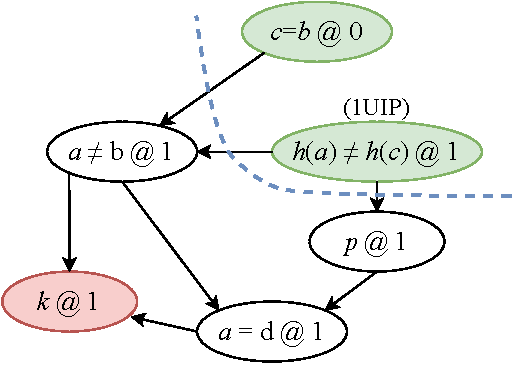
\includegraphics[width=0.35\linewidth]{./img/_conflict_graph_example.pdf}
    \end{center}
    A cut in front of the 1UIP that separates decision nodes and the conflict node (as in standard CDCL) is made
    to obtain the conflict set $\eta = \{ h(a) \neq h(c), c = b \}$.
    $\big( (h(a) = h(c)) \vee (c \neq b) \big)$ is added as a clause and the algorithm backjumps at the decision level 0.
\end{example}

